\documentclass{IEEEtran}

\usepackage{graphicx}
\usepackage{caption}
\usepackage{subcaption}
\usepackage{hyperref}
\usepackage{url}

\bibliographystyle{plain}

\begin{document}

\title{Computational Psycholinguistics --- Assignment 2}
\author{Daan Brugmans (S1080742)}
\date{\today}

\graphicspath{{./images}}

\maketitle

\section{Introduction}
This report is the realization of the Assignment 2 project for the Radboud University course \href{https://www.ru.nl/courseguides/arts/courses/ma/rema-lc/let-rema-lcex28/}{Computational Psycholinguistics}.
For this assignment, students must investigate whether the gradients computed from a recurrent neural network correlate with measured P600 component activity from a controlled experiment.
The reasoning behind this assignment is that recent research (\cite{fitz2019erp,frank2024gradients}) has shown that the P600 component may be the backpropagation of prediction errors in the human language system.
Since neural language models also backpropagate their prediction errors using gradients, there may exist similarities between the language error backpropagation of human and artificial neural language systems.
This report contains the findings found by me for the Assignment 2 project.

The relevant code for this assignment can be found at the following URL: \url{https://github.com/daanbrugmans/ru-computational-psycholinguistics-23-24/tree/main/assignment-2/code}.

\section{Related Work}
For the Assignment 2 project, students must choose a controlled experiment where participants read English or Dutch sentences while their P600 component is measured.
I have chosen to use the data from the controlled experiment performed in \cite{frank2015erp}.
This data is also used by the authors of \cite{frank2024gradients}, and is briefly introduced in the description of the Assignment 2 project.
This means that my report is (an attempt at) an extension of the work in \cite{frank2024gradients}.

The data from the controlled experiment in \cite{frank2015erp} consists of EEG data of 24 native British English speakers, who all read a set of 205 sentences taken from English-language novels.
The authors recorded EEG data of six different ERP components, including the P600 component, and calculated the average EEG values for every ERP component, for every word of every sentence for every participant of the experiment.
This dataset should fulfill the requirements set by the assignment: the experiment language is English, the participants' stimuli are independent sentences, the size of the P600 component is one dependent variable and showed an effect, and the independent variables are manipulated by varying the content of the sentence stimuli.

\section{Methodology}
All the code I have written can be found in the Jupyter Notebook called \texttt{main.ipynb}, which should thusly contain all results also shown in this report.
It can be found at the following URL: \url{https://github.com/daanbrugmans/ru-computational-psycholinguistics-23-24/blob/main/assignment-2/code/main.ipynb}
I have placed the code in the \texttt{get\_predictions.py} file in a function called \texttt{get\_predictions}, so that I can easily call this code from the notebook.

The dataset of the study in \cite{frank2015erp} is openly accessible through a collection of \texttt{.mat} files, which are typically used in a MatLab setting, but I use Scipy to open this data.
Within the collection of code I hand in alongside this report, the raw data file I used for my experiment can be found in the \texttt{data} folder as \texttt{code/data/stimuli\_erp.mat}.
The original README provided by the authors is also included.
From this dataset, I collect the list of sentences read by the participants of the study, and the related ERP data.
Although this data does not need any preprocessing, I do wrangle the ERP data into the format used by the code in \texttt{get\_predictions.py}, so that I can easily merge the data from the study with the data generated by the models.
I also write the sentence data from the study to a plain text file in the \texttt{items} folder called \texttt{stimuli.txt}, as is required for generating model results.

The data from \cite{frank2015erp} includes the P600 component for all 24 participants per word.
I have chosen to take the mean of all 24 P600s and only analyse these means.
I made this decision because I wanted to have a single P600 for every word to represent the entire participant population.
I have chosen the mean as opposed to the median because of its sensitivity to outliers: I wanted to include information about participants with outlying P600 values for specific words into the aggregated P600 value, and I think that the mean does a better job at this than the median due to its sensitivity to outliers.

My results are a collection of scatterplots that visualize the relationship between 3 variables on the sentence data: the Mean P600 Component, the Surprisal of a Model, and the Gradient Values of a Model.
Every plot also contains a quadratic function fitted to the data to show the trend of the relationship between the variables.
I have chosen for a quadratic function as opposed to a linear function, as I found that this fits the data better.
Included in every plot is also the Pearson Correlation Coefficient \textit{r} between variables.
Since surprisal values and gradients are calculated for multiple models, I provide a plot for every model.
For every pair of variables, I also provide a plot of how the Pearson Correlation Coefficient changes as the model is trained on more data, which will be the main focus of my results.

Before producing results, I set a universal seed for Python itself, NumPy, and PyTorch of \texttt{3131}.
I do this in order to improve the reproducibility of my results.
This is why I also set some settings for CUDA regarding PyTorch's randomness when computing on GPU.

\section{Results}
\begin{figure*}
    \centering
    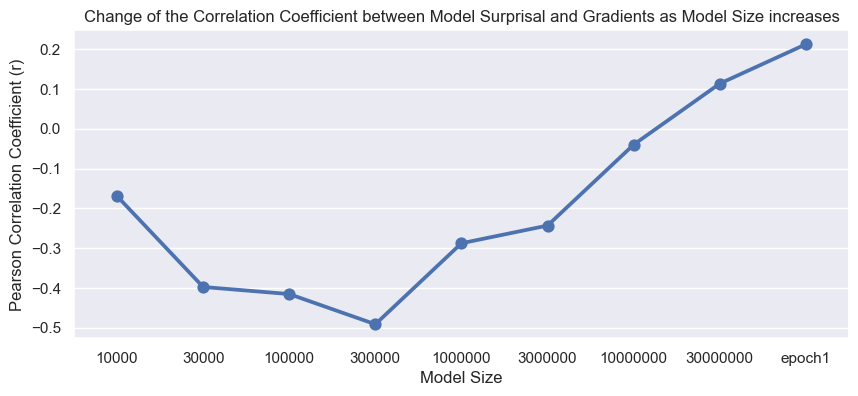
\includegraphics[width=.9\textwidth]{correlation_change/surprisal_gradients.png}
    \caption{The change of the Pearson Correlation Coefficient between Model Surprisal and Model Gradients as the model is trained on increasingly more data.}
    \label{fig:coefficient_surprisal_gradients}
\end{figure*}
\begin{figure*}
    \centering
    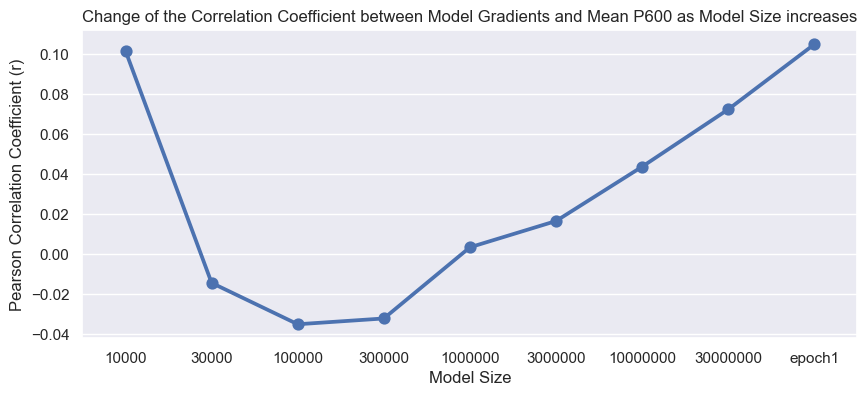
\includegraphics[width=.9\textwidth]{correlation_change/gradients_p600.png}
    \caption{The change of the Pearson Correlation Coefficient between Model Gradients and P600 as the model is trained on increasingly more data.}
    \label{fig:coefficient_gradients_p600}
\end{figure*}
\begin{figure*}
    \centering
    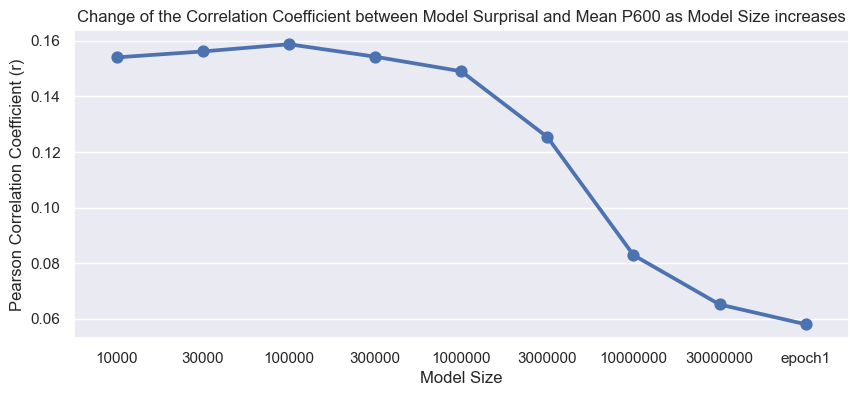
\includegraphics[width=.9\textwidth]{correlation_change/surprisal_p600.png}
    \caption{The change of the Pearson Correlation Coefficient between Model Surprisal and Mean P600 as the model is trained on increasingly more data.}
    \label{fig:coefficient_surprisal_p600}
\end{figure*}

Figures \ref{fig:coefficient_surprisal_gradients}, \ref{fig:coefficient_gradients_p600}, and \ref{fig:coefficient_surprisal_p600} show the change of the correlation between variables as the amount of data the neural language model has trained on increases.
The exact values of the points in this plot can be found in tables \ref{tab:correlation_surprisal_gradients}, \ref{tab:correlation_gradients_p600}, and \ref{tab:correlation_surprisal_p600} respectively.
The individual scatterplots are placed in the appendices.

\section{Discussion}
The data in figure \ref{fig:coefficient_surprisal_gradients} show an interesting trend in the predictive power of a model's surprisal for its gradients: the strength of the correlation between the variables gets stronger as the model has trained on more data.
This strength reaches a peak when the model is trained on 300,000 sentences, after which, the correlation strength starts to move into the opposite direction; it returns to zero and grows from negative to positive.
I expect that the increasing strength of the correlation until 300,000 sentences can be explained by the learning process of the model.
As the model has learned more, its gradients become a better representation of its surprisal, because it has gained an understanding of the data it has learned.
When it has reached this depth of understanding, words that it expects backpropagate with small losses, while words that it is surprised by backpropagate with large losses.
As the model continues to learn, the surprisal starts to become a worse predictor of the gradients.
I expect this is due to overfitting: the model doesn't learn from being surprised by words anymore, so the backpropagated losses represent other information that it is learning.
Since these losses represent more than just surprisal, they become less correlated with surprisal.

When familiar with the trend shown in figure \ref{fig:coefficient_surprisal_gradients}, the results of figure \ref{tab:correlation_gradients_p600} become interesting: both figures show the same trend of the correlation changing over time.
That is, the correlation between the model's gradients and the model's surprisal, and the correlation between the model's gradients and the mean P600, follow the trend that the correlation decreases until 300,000 sentences, after which the correlation starts to grow into the positives.
However, while the correlation strength between Model Surprisal and Gradients is at its strongest at 300,000 sentences, this does not hold for the correlation between Model Surprisal and Mean P600, which actually reaches a peak after a full epoch of training.
If we assume my explanation about the change in correlation between Model Surprisal and Gradients being caused by the model learning more than just surprisal to be true, then the fact that the correlation between Model Gradients and Mean P600 reaches a peak after a fully trained model may mean that the model's gradients are best at predicting Mean P600 values when the model has learned to use more than just surprisal when backpropagating errors.
This, in turn, would imply that just surprisal would not be a strong predictor of the P600 component.
I would even state that this means that the P600 component may be more than just the backpropagation of surprisal in humans, although I do make this claim as someone not well-versed in psycholinguistics.

Figure \ref{fig:coefficient_surprisal_p600} seems to show a clear picture: as the amount of data the model has been trained on increases, the correlation between Model Surprisal and Mean P600 decreases, and surprisal increasingly becomes a worse predictor of the P600 component.
I think that this development is caused by the scale of the data that the model has been trained on: once the model has been trained on millions of sentences, or even tens of millions, the correlation decreases because the model's surprisal grows to reflect a human's backpropagation worse.
The model has learned on so much data that it is not surprised anymore by things that a regular human would have to backpropagate on.
This phenomenon has also been shown to exist in other large language models, such as modern transformers (\cite{oh2023why}).

\begin{table}
    \centering
    \begin{tabular}{c|c}
        \textbf{Trained Data Count} & \textbf{\textit{r}} \\
        \hline
        10000&-0.169\\
        30000&-0.397\\
        100000&-0.415\\
        300000&-0.491\\
        1000000&-0.288\\
        3000000&-0.243\\
        10000000&-0.040\\
        30000000&0.113\\
        epoch1&0.212
    \end{tabular}
    \caption{Correlation Coefficients between Model Surprisal and Model Gradients by the model's train data size.}
    \label{tab:correlation_surprisal_gradients}
\end{table}
\begin{table}
    \centering
    \begin{tabular}{c|c}
        \textbf{Trained Data Count} & \textbf{\textit{r}} \\
        \hline
        10000&0.103\\
        30000&-0.026\\
        100000&-0.035\\
        300000&-0.037\\
        1000000&0.007\\
        3000000&0.021\\
        10000000&0.053\\
        30000000&0.084\\
        epoch1&0.116
    \end{tabular}
    \caption{Correlation Coefficients between Model Gradients and Mean P600 by the model's train data size.}
    \label{tab:correlation_gradients_p600}
\end{table}
\begin{table}
    \centering
    \begin{tabular}{c|c}
        \textbf{Trained Data Count} & \textbf{\textit{r}} \\
        \hline
        10000&0.154\\
        30000&0.156\\
        100000&0.159\\
        300000&0.154\\
        1000000&0.149\\
        3000000&0.125\\
        10000000&0.083\\
        30000000&0.065\\
        epoch1&0.058
    \end{tabular}
    \caption{Correlation Coefficients between Model Surprisal and Mean P600 by the model's train data size.}
    \label{tab:correlation_surprisal_p600}
\end{table}

\section{Conclusions}
From my findings, I would conclude that the P600 component is marginally simulated by model surprisal, but only for models trained on 100,000 sentences or less.
Bigger models seem to become worse predictors of the P600, which is likely due to the scale of the data they were trained on, causing the models' surprisal values to reflect those of humans worse.
Regardless, the strongest correlation between Model Surprisal and the P600 component is still only 0.159, which is quite weak.
The Model Gradients seem to be even weaker predictors of P600 values, and, on the basis of my findings, I would conclude that they do not explain the P600 component.

\bibliography{bib}

\onecolumn
\appendix
\section*{Appendix A: Plots of Model Surprisal vs. Model Gradients}
\begin{figure*}[h]
    \centering
    \begin{subfigure}{0.4\textwidth}
        \centering
        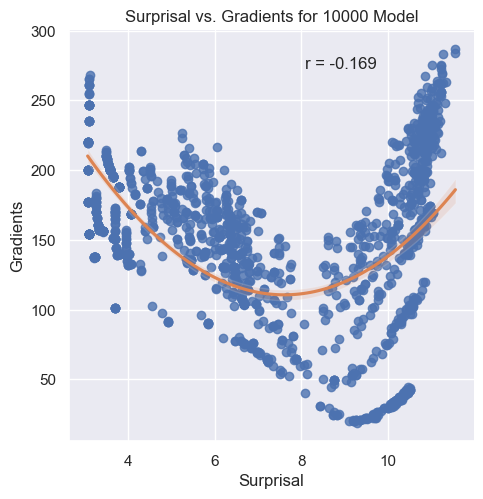
\includegraphics[width=\textwidth]{surprisal_vs_gradients/10000.png}
    \end{subfigure}
    \begin{subfigure}{0.4\textwidth}
        \centering
        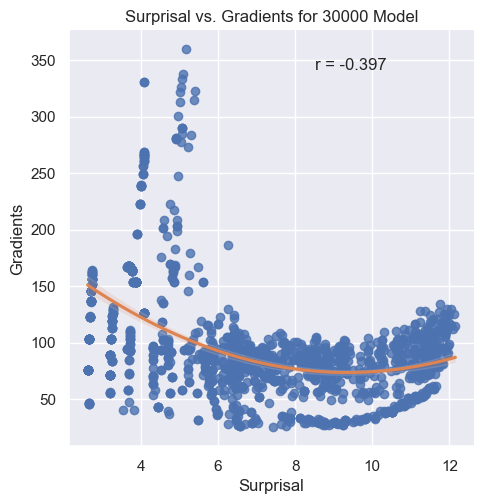
\includegraphics[width=\textwidth]{surprisal_vs_gradients/30000.png}
    \end{subfigure}
\end{figure*}
\begin{figure*}[h]
\centering
\begin{subfigure}{0.4\textwidth}
    \centering
    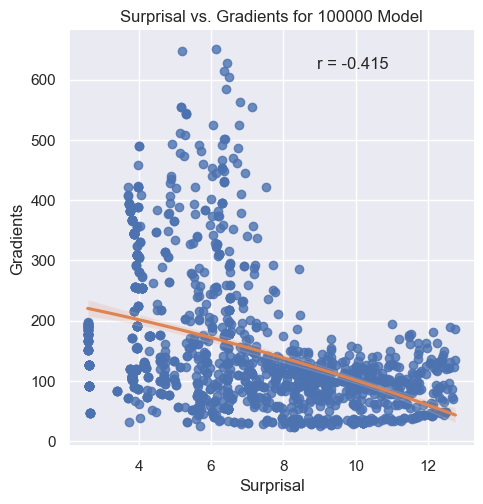
\includegraphics[width=\textwidth]{surprisal_vs_gradients/100000.png}
\end{subfigure}
\begin{subfigure}{0.4\textwidth}
    \centering
    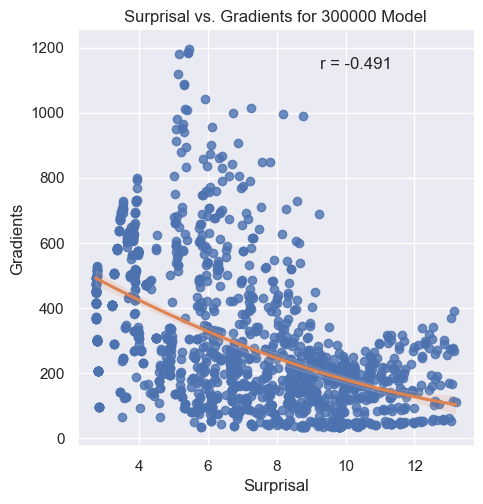
\includegraphics[width=\textwidth]{surprisal_vs_gradients/300000.png}
\end{subfigure}
\end{figure*}
\begin{figure*}[h]
    \centering
    \begin{subfigure}{0.4\textwidth}
        \centering
        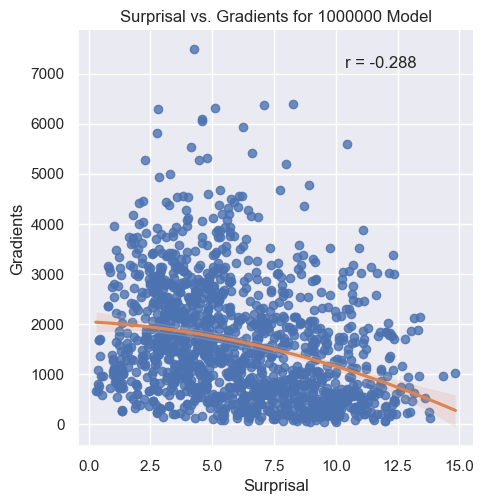
\includegraphics[width=\textwidth]{surprisal_vs_gradients/1000000.png}
    \end{subfigure}
    \begin{subfigure}{0.4\textwidth}
        \centering
        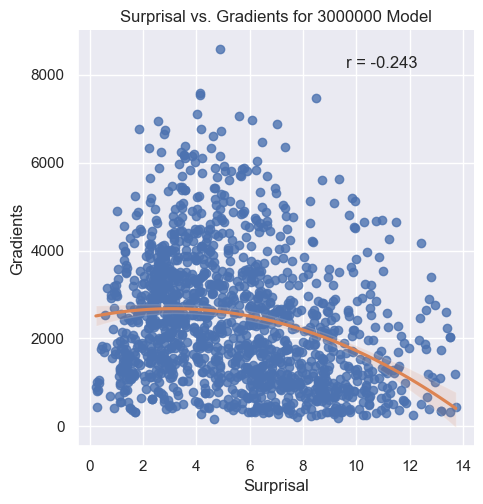
\includegraphics[width=\textwidth]{surprisal_vs_gradients/3000000.png}
    \end{subfigure}
\end{figure*}
\begin{figure*}[h]
    \centering
    \begin{subfigure}{0.4\textwidth}
        \centering
        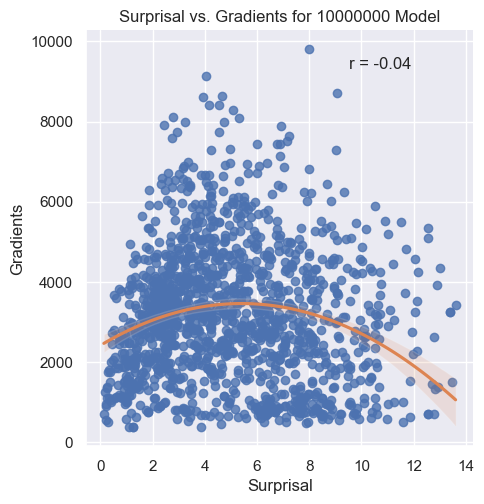
\includegraphics[width=\textwidth]{surprisal_vs_gradients/10000000.png}
    \end{subfigure}
    \begin{subfigure}{0.4\textwidth}
        \centering
        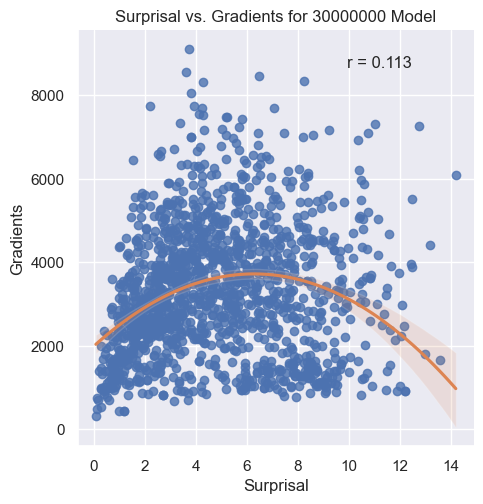
\includegraphics[width=\textwidth]{surprisal_vs_gradients/30000000.png}
    \end{subfigure}
\end{figure*}
\begin{figure*}[h]
    \centering
    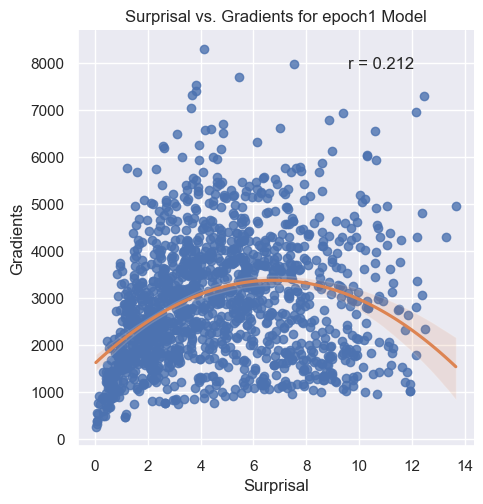
\includegraphics[width=0.4\textwidth]{surprisal_vs_gradients/epoch1.png}
\end{figure*}

\clearpage

\section*{Appendix B: Plots of Model Gradients vs. Mean P600 Component}
\begin{figure*}[h]
    \centering
    \begin{subfigure}{0.4\textwidth}
        \centering
        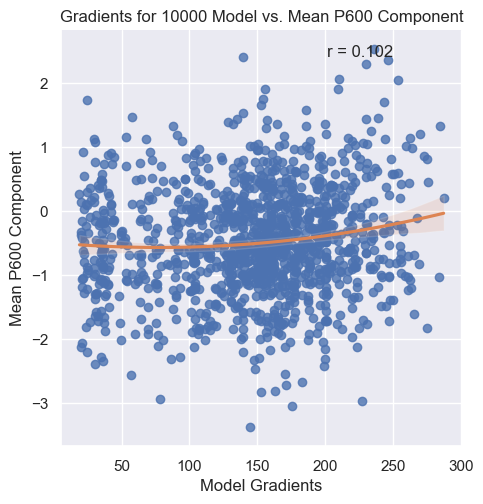
\includegraphics[width=\textwidth]{gradients_vs_p600/10000.png}
    \end{subfigure}
    \begin{subfigure}{0.4\textwidth}
        \centering
        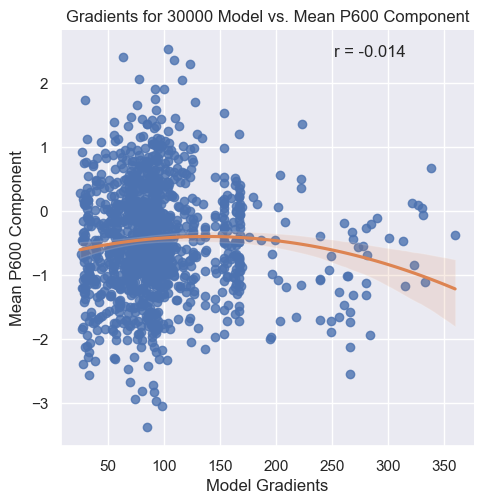
\includegraphics[width=\textwidth]{gradients_vs_p600/30000.png}
    \end{subfigure}
\end{figure*}
\begin{figure*}[h]
\centering
\begin{subfigure}{0.4\textwidth}
    \centering
    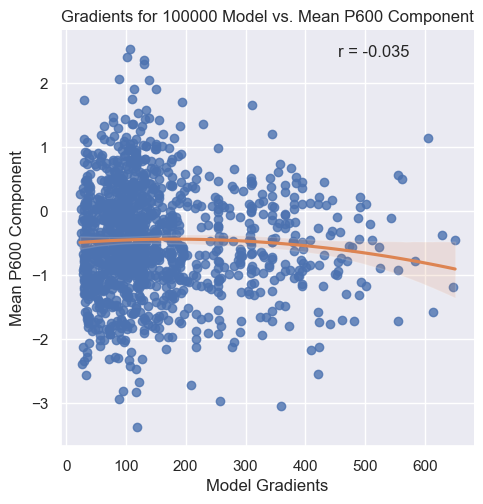
\includegraphics[width=\textwidth]{gradients_vs_p600/100000.png}
\end{subfigure}
\begin{subfigure}{0.4\textwidth}
    \centering
    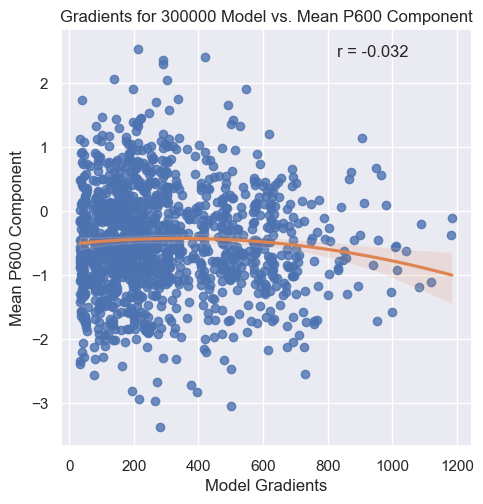
\includegraphics[width=\textwidth]{gradients_vs_p600/300000.png}
\end{subfigure}
\end{figure*}
\begin{figure*}[h]
    \centering
    \begin{subfigure}{0.4\textwidth}
        \centering
        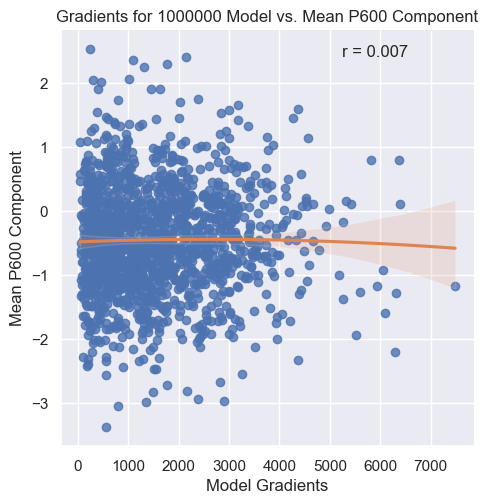
\includegraphics[width=\textwidth]{gradients_vs_p600/1000000.png}
    \end{subfigure}
    \begin{subfigure}{0.4\textwidth}
        \centering
        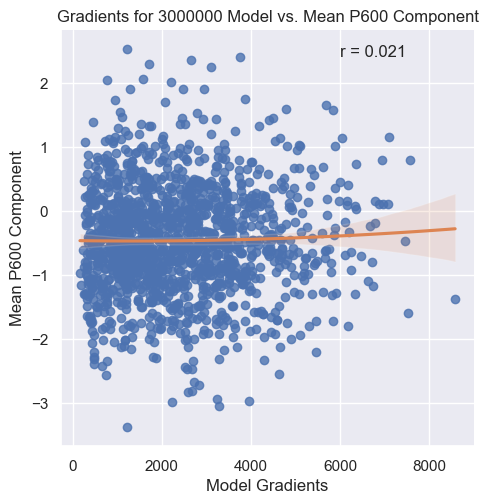
\includegraphics[width=\textwidth]{gradients_vs_p600/3000000.png}
    \end{subfigure}
\end{figure*}
\begin{figure*}[h]
    \centering
    \begin{subfigure}{0.4\textwidth}
        \centering
        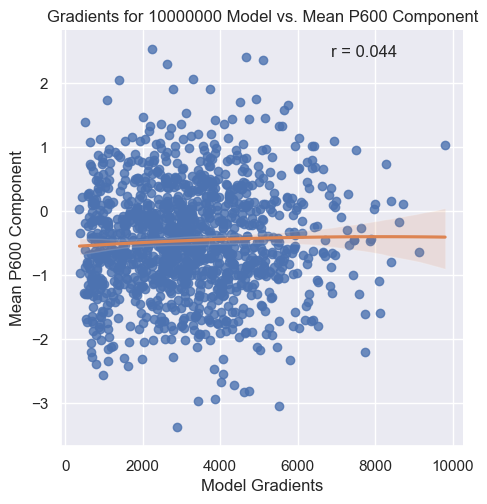
\includegraphics[width=\textwidth]{gradients_vs_p600/10000000.png}
    \end{subfigure}
    \begin{subfigure}{0.4\textwidth}
        \centering
        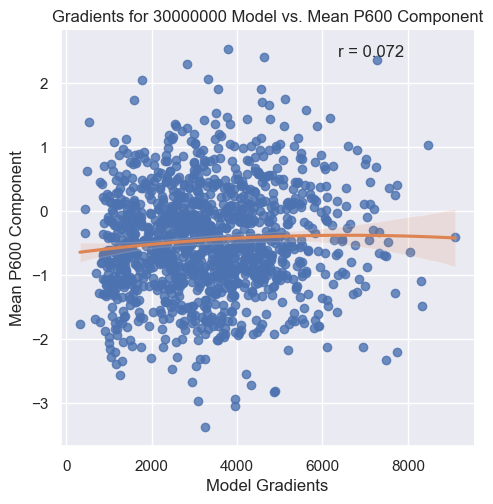
\includegraphics[width=\textwidth]{gradients_vs_p600/30000000.png}
    \end{subfigure}
\end{figure*}
\begin{figure*}[h]
    \centering
    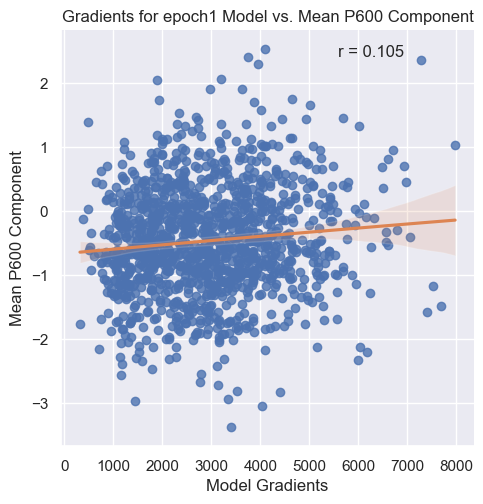
\includegraphics[width=0.4\textwidth]{gradients_vs_p600/epoch1.png}
\end{figure*}

\clearpage

\section*{Appendix C: Plots of Model Surprisal vs. Mean P600 Component}
\begin{figure*}[h]
    \centering
    \begin{subfigure}{0.4\textwidth}
        \centering
        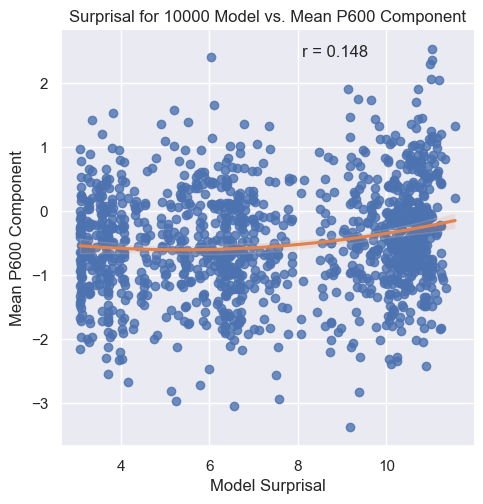
\includegraphics[width=\textwidth]{surprisal_vs_p600/10000.png}
    \end{subfigure}
    \begin{subfigure}{0.4\textwidth}
        \centering
        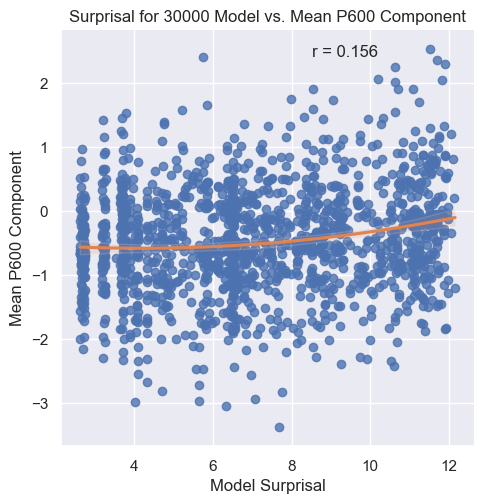
\includegraphics[width=\textwidth]{surprisal_vs_p600/30000.png}
    \end{subfigure}
\end{figure*}
\begin{figure*}[h]
\centering
\begin{subfigure}{0.4\textwidth}
    \centering
    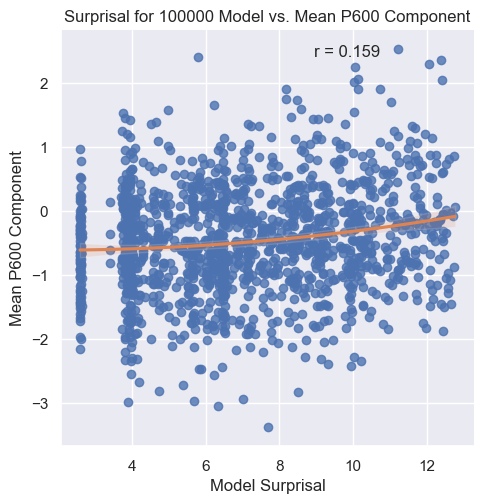
\includegraphics[width=\textwidth]{surprisal_vs_p600/100000.png}
\end{subfigure}
\begin{subfigure}{0.4\textwidth}
    \centering
    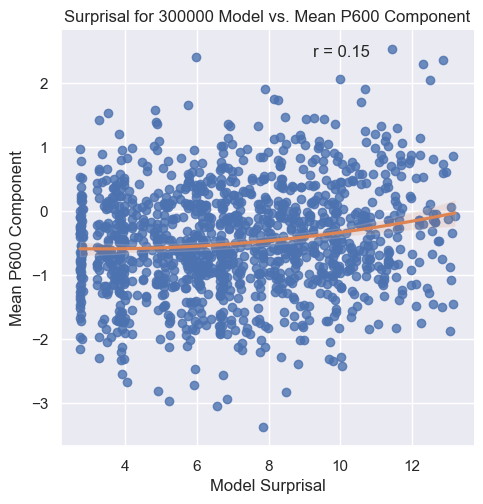
\includegraphics[width=\textwidth]{surprisal_vs_p600/300000.png}
\end{subfigure}
\end{figure*}
\begin{figure*}[h]
    \centering
    \begin{subfigure}{0.4\textwidth}
        \centering
        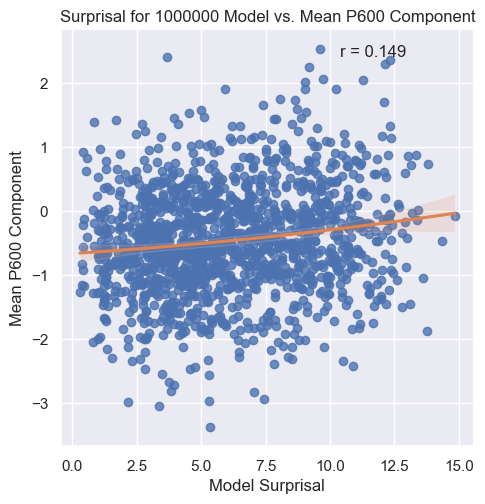
\includegraphics[width=\textwidth]{surprisal_vs_p600/1000000.png}
    \end{subfigure}
    \begin{subfigure}{0.4\textwidth}
        \centering
        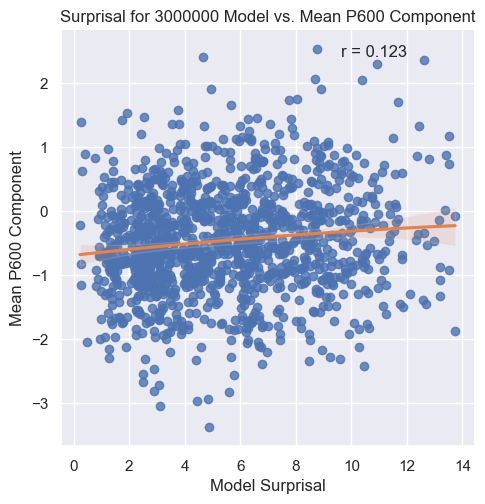
\includegraphics[width=\textwidth]{surprisal_vs_p600/3000000.png}
    \end{subfigure}
\end{figure*}
\begin{figure*}[h]
    \centering
    \begin{subfigure}{0.4\textwidth}
        \centering
        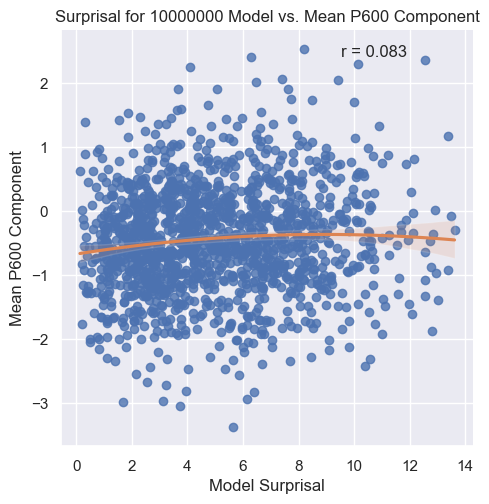
\includegraphics[width=\textwidth]{surprisal_vs_p600/10000000.png}
    \end{subfigure}
    \begin{subfigure}{0.4\textwidth}
        \centering
        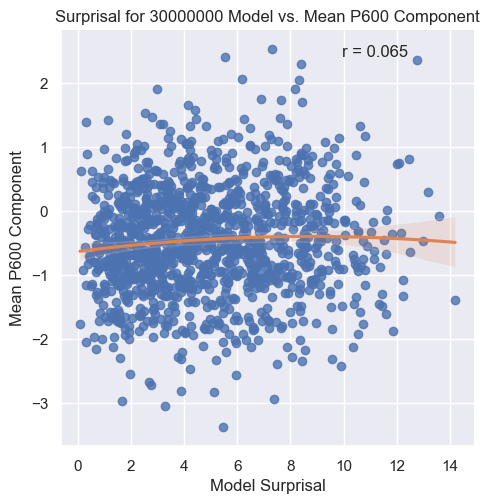
\includegraphics[width=\textwidth]{surprisal_vs_p600/30000000.png}
    \end{subfigure}
\end{figure*}
\begin{figure*}[h]
    \centering
    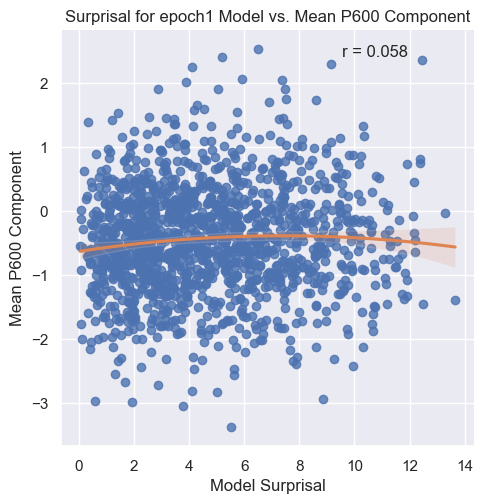
\includegraphics[width=0.4\textwidth]{surprisal_vs_p600/epoch1.png}
\end{figure*}

\end{document}